% ── Section 6: Results ────────────────────────────────────────────────────────
\section{Results}
\label{sec:results}

% NOTE TO AUTHOR:
% Replace every \TODO{X.XX} with the actual number after running experiments.
% Run scripts in this order:
%   evaluation/01_run_baselines.py
%   evaluation/02_run_finetuned.py
%   evaluation/09_lm_shallow_fusion.py --tune_alpha
%   evaluation/10_whisper_size_comparison.py
%   evaluation/03_compute_metrics.py
%   Then copy numbers from evaluation/results/all_metrics_summary.json

\subsection{Main Results}

Table~\ref{tab:main_results} presents WER, CER, MIX-ER, and CS-Detection
F1 for all models on the BanglaMix test set.

\begin{table*}[ht]
\centering
\caption{
  Main results on the BanglaMix test set.
  WER/CER: lower is better. CS-F1: higher is better.
  \BEST{Bold green} = best overall.
  $\dagger$ = statistically significant improvement over Whisper large-v3
  zero-shot ($p < 0.05$, paired bootstrap).
}
\label{tab:main_results}
\small
\setlength{\tabcolsep}{5pt}
\begin{tabular}{llrrrrrrr}
\toprule
& \textbf{Model}
  & \textbf{WER}$\downarrow$
  & \textbf{CER}$\downarrow$
  & \textbf{WER-BN}$\downarrow$
  & \textbf{WER-EN}$\downarrow$
  & \textbf{MIX-ER}$\downarrow$
  & \textbf{WER-CS}$\downarrow$
  & \textbf{CS-F1}$\uparrow$ \\
\midrule
\multicolumn{9}{l}{\textit{Zero-shot baselines (no fine-tuning on BanglaMix)}} \\
\midrule
& Whisper large-v3        & \TODO{0.XX} & \TODO{0.XX} & \TODO{0.XX} & \TODO{0.XX} & \TODO{0.XX} & \TODO{0.XX} & \TODO{0.XX} \\
& Tugstugi/whisper-bn     & \TODO{0.XX} & \TODO{0.XX} & \TODO{0.XX} & \TODO{0.XX} & \TODO{0.XX} & \TODO{0.XX} & \TODO{0.XX} \\
& MMS-1B                  & \TODO{0.XX} & \TODO{0.XX} & \TODO{0.XX} & \TODO{0.XX} &     ---     & \TODO{0.XX} & \TODO{0.XX} \\
& wav2vec2-XLS-R-BN       & \TODO{0.XX} & \TODO{0.XX} & \TODO{0.XX} & \TODO{0.XX} &     ---     & \TODO{0.XX} & \TODO{0.XX} \\
\midrule
\multicolumn{9}{l}{\textit{CTC models fine-tuned on BanglaMix}} \\
\midrule
& wav2vec2 (no LM)        & \TODO{0.XX} & \TODO{0.XX} & \TODO{0.XX} & \TODO{0.XX} & \TODO{0.XX} & \TODO{0.XX} & \TODO{0.XX} \\
& wav2vec2 + 5-gram LM$^\dagger$   & \TODO{0.XX} & \TODO{0.XX} & \TODO{0.XX} & \TODO{0.XX} & \TODO{0.XX} & \TODO{0.XX} & \TODO{0.XX} \\
& WavLM (no LM)           & \TODO{0.XX} & \TODO{0.XX} & \TODO{0.XX} & \TODO{0.XX} & \TODO{0.XX} & \TODO{0.XX} & \TODO{0.XX} \\
& WavLM + 5-gram LM$^\dagger$      & \TODO{0.XX} & \TODO{0.XX} & \TODO{0.XX} & \TODO{0.XX} & \TODO{0.XX} & \TODO{0.XX} & \TODO{0.XX} \\
\midrule
\multicolumn{9}{l}{\textit{Whisper fine-tuned on BanglaMix --- ablation}} \\
\midrule
& Whisper FT BN\_ONLY (A) & \TODO{0.XX} & \TODO{0.XX} & \TODO{0.XX} & \TODO{0.XX} & \TODO{0.XX} & \TODO{0.XX} & \TODO{0.XX} \\
& Whisper FT CS\_ONLY (B) & \TODO{0.XX} & \TODO{0.XX} & \TODO{0.XX} & \TODO{0.XX} & \TODO{0.XX} & \TODO{0.XX} & \TODO{0.XX} \\
& \BEST{Whisper FT ALL (Proposed)$^\dagger$} & \BEST{\TODO{0.XX}} & \BEST{\TODO{0.XX}} & \BEST{\TODO{0.XX}} & \BEST{\TODO{0.XX}} & \BEST{\TODO{0.XX}} & \BEST{\TODO{0.XX}} & \BEST{\TODO{0.XX}} \\
\bottomrule
\end{tabular}
\end{table*}

\paragraph{Key findings.}

\begin{itemize}[leftmargin=*, itemsep=2pt]
  \item \textbf{Zero-shot baselines underperform significantly on dialectal CS.}
        Whisper large-v3, despite being trained on 680k~hours, achieves a WER
        of \TODO{XX.X}\% on our test set, confirming that multilingual
        pre-training alone does not generalise to dialectal CS.
  \item \textbf{Tugstugi (dialect, no CS) vs.\ our model (dialect + CS).}
        Tugstugi achieves lower WER-BN than the zero-shot Whisper (it has seen
        dialectal Bengali) but much higher WER-EN (it has never seen CS), leading
        to a higher MIX-ER. This quantifies the cost of ignoring CS in training.
  \item \textbf{LM shallow fusion improves CTC models.}
        Adding a 5-gram LM (optimal $\alpha$=\TODO{X.X}, $\beta$=\TODO{X.X})
        reduces WER of wav2vec2 by a relative \TODO{XX.X}\% and WavLM by
        \TODO{XX.X}\%, confirming the benefit of external LM knowledge.
  \item \textbf{Ablation: ALL $>$ CS\_ONLY $>$ BN\_ONLY.}
        Training on only BN\_ONLY achieves the worst WER-EN (the model never
        sees CS). Training on only CS\_ONLY achieves good WER-EN but higher
        WER-BN (less dialect variety). The combined ALL training yields the
        best performance across all metrics.
  \item \textbf{Proposed system achieves \TODO{XX.X}\% relative WER reduction}
        over the strongest baseline (Tugstugi), statistically significant at
        $p < 0.01$ with a Cohen's~$d$ of \TODO{X.XX} (large effect).
\end{itemize}

\subsection{Whisper Model Size Comparison}

Table~\ref{tab:size_comparison} shows WER and CER for all five Whisper sizes
in zero-shot and fine-tuned conditions.

\begin{table}[h]
\centering
\caption{Whisper model size comparison on BanglaMix test set.
RTF = Real-Time Factor (lower = faster). Measured on A100 GPU.}
\label{tab:size_comparison}
\small
\begin{tabular}{lrrrrr}
\toprule
\textbf{Model} & \textbf{Params} & \multicolumn{2}{c}{\textbf{Zero-shot}} & \multicolumn{2}{c}{\textbf{Fine-tuned}} \\
\cmidrule(lr){3-4}\cmidrule(lr){5-6}
& & WER & CER & WER & CER \\
\midrule
tiny   &  39M & \TODO{0.XX} & \TODO{0.XX} & \TODO{0.XX} & \TODO{0.XX} \\
base   &  74M & \TODO{0.XX} & \TODO{0.XX} & \TODO{0.XX} & \TODO{0.XX} \\
small  & 244M & \TODO{0.XX} & \TODO{0.XX} & \TODO{0.XX} & \TODO{0.XX} \\
medium & 769M & \TODO{0.XX} & \TODO{0.XX} & \TODO{0.XX} & \TODO{0.XX} \\
large-v3 & 1550M & \TODO{0.XX} & \TODO{0.XX} & \BEST{\TODO{0.XX}} & \BEST{\TODO{0.XX}} \\
\bottomrule
\end{tabular}
\end{table}

\subsection{LM Tuning Results}

Grid search over $\alpha$ and $\beta$ on the development set (200 clips)
yields optimal values of $\alpha^* = \TODO{X.X}$, $\beta^* = \TODO{X.X}$
for wav2vec2 and $\alpha^* = \TODO{X.X}$, $\beta^* = \TODO{X.X}$ for WavLM.
Development WER decreases from \TODO{0.XX} (greedy) to \TODO{0.XX} (LM fusion)
for wav2vec2, confirming that LM integration is beneficial.

\subsection{Per-Dialect WER}

Figure~\ref{fig:dialect_heatmap} shows the model $\times$ dialect WER heatmap.
Full per-dialect results for the proposed system are in
Table~\ref{tab:per_dialect}.

\begin{table}[h]
\centering
\caption{Per-dialect WER for the proposed model (Whisper FT ALL).}
\label{tab:per_dialect}
\small
\begin{tabular}{lrrr}
\toprule
\textbf{Dialect} & \textbf{Clips} & \textbf{WER}$\downarrow$ & \textbf{CER}$\downarrow$ \\
\midrule
Sylhet       & \TODO{XXX} & \TODO{0.XX} & \TODO{0.XX} \\
Old\_Dhaka   & \TODO{XXX} & \TODO{0.XX} & \TODO{0.XX} \\
Sandwip      & \TODO{XXX} & \TODO{0.XX} & \TODO{0.XX} \\
Barishal     & \TODO{XXX} & \TODO{0.XX} & \TODO{0.XX} \\
Chittagong   & \TODO{XXX} & \TODO{0.XX} & \TODO{0.XX} \\
Khulna       & \TODO{XXX} & \TODO{0.XX} & \TODO{0.XX} \\
Kishoreganj  & \TODO{XXX} & \TODO{0.XX} & \TODO{0.XX} \\
Comilla      & \TODO{XXX} & \TODO{0.XX} & \TODO{0.XX} \\
Narail       & \TODO{XXX} & \TODO{0.XX} & \TODO{0.XX} \\
Rangpur      & \TODO{XXX} & \TODO{0.XX} & \TODO{0.XX} \\
Narsingdi    & \TODO{XXX} & \TODO{0.XX} & \TODO{0.XX} \\
Mymensingh   & \TODO{XXX} & \TODO{0.XX} & \TODO{0.XX} \\
Habiganj     & \TODO{XXX} & \TODO{0.XX} & \TODO{0.XX} \\
Tangail      & \TODO{XXX} & \TODO{0.XX} & \TODO{0.XX} \\
Noakhali     & \TODO{XXX} & \TODO{0.XX} & \TODO{0.XX} \\
\midrule
\textbf{Overall} & \TODO{5100} & \BEST{\TODO{0.XX}} & \BEST{\TODO{0.XX}} \\
\bottomrule
\end{tabular}
\end{table}

\begin{figure}[h]
\centering
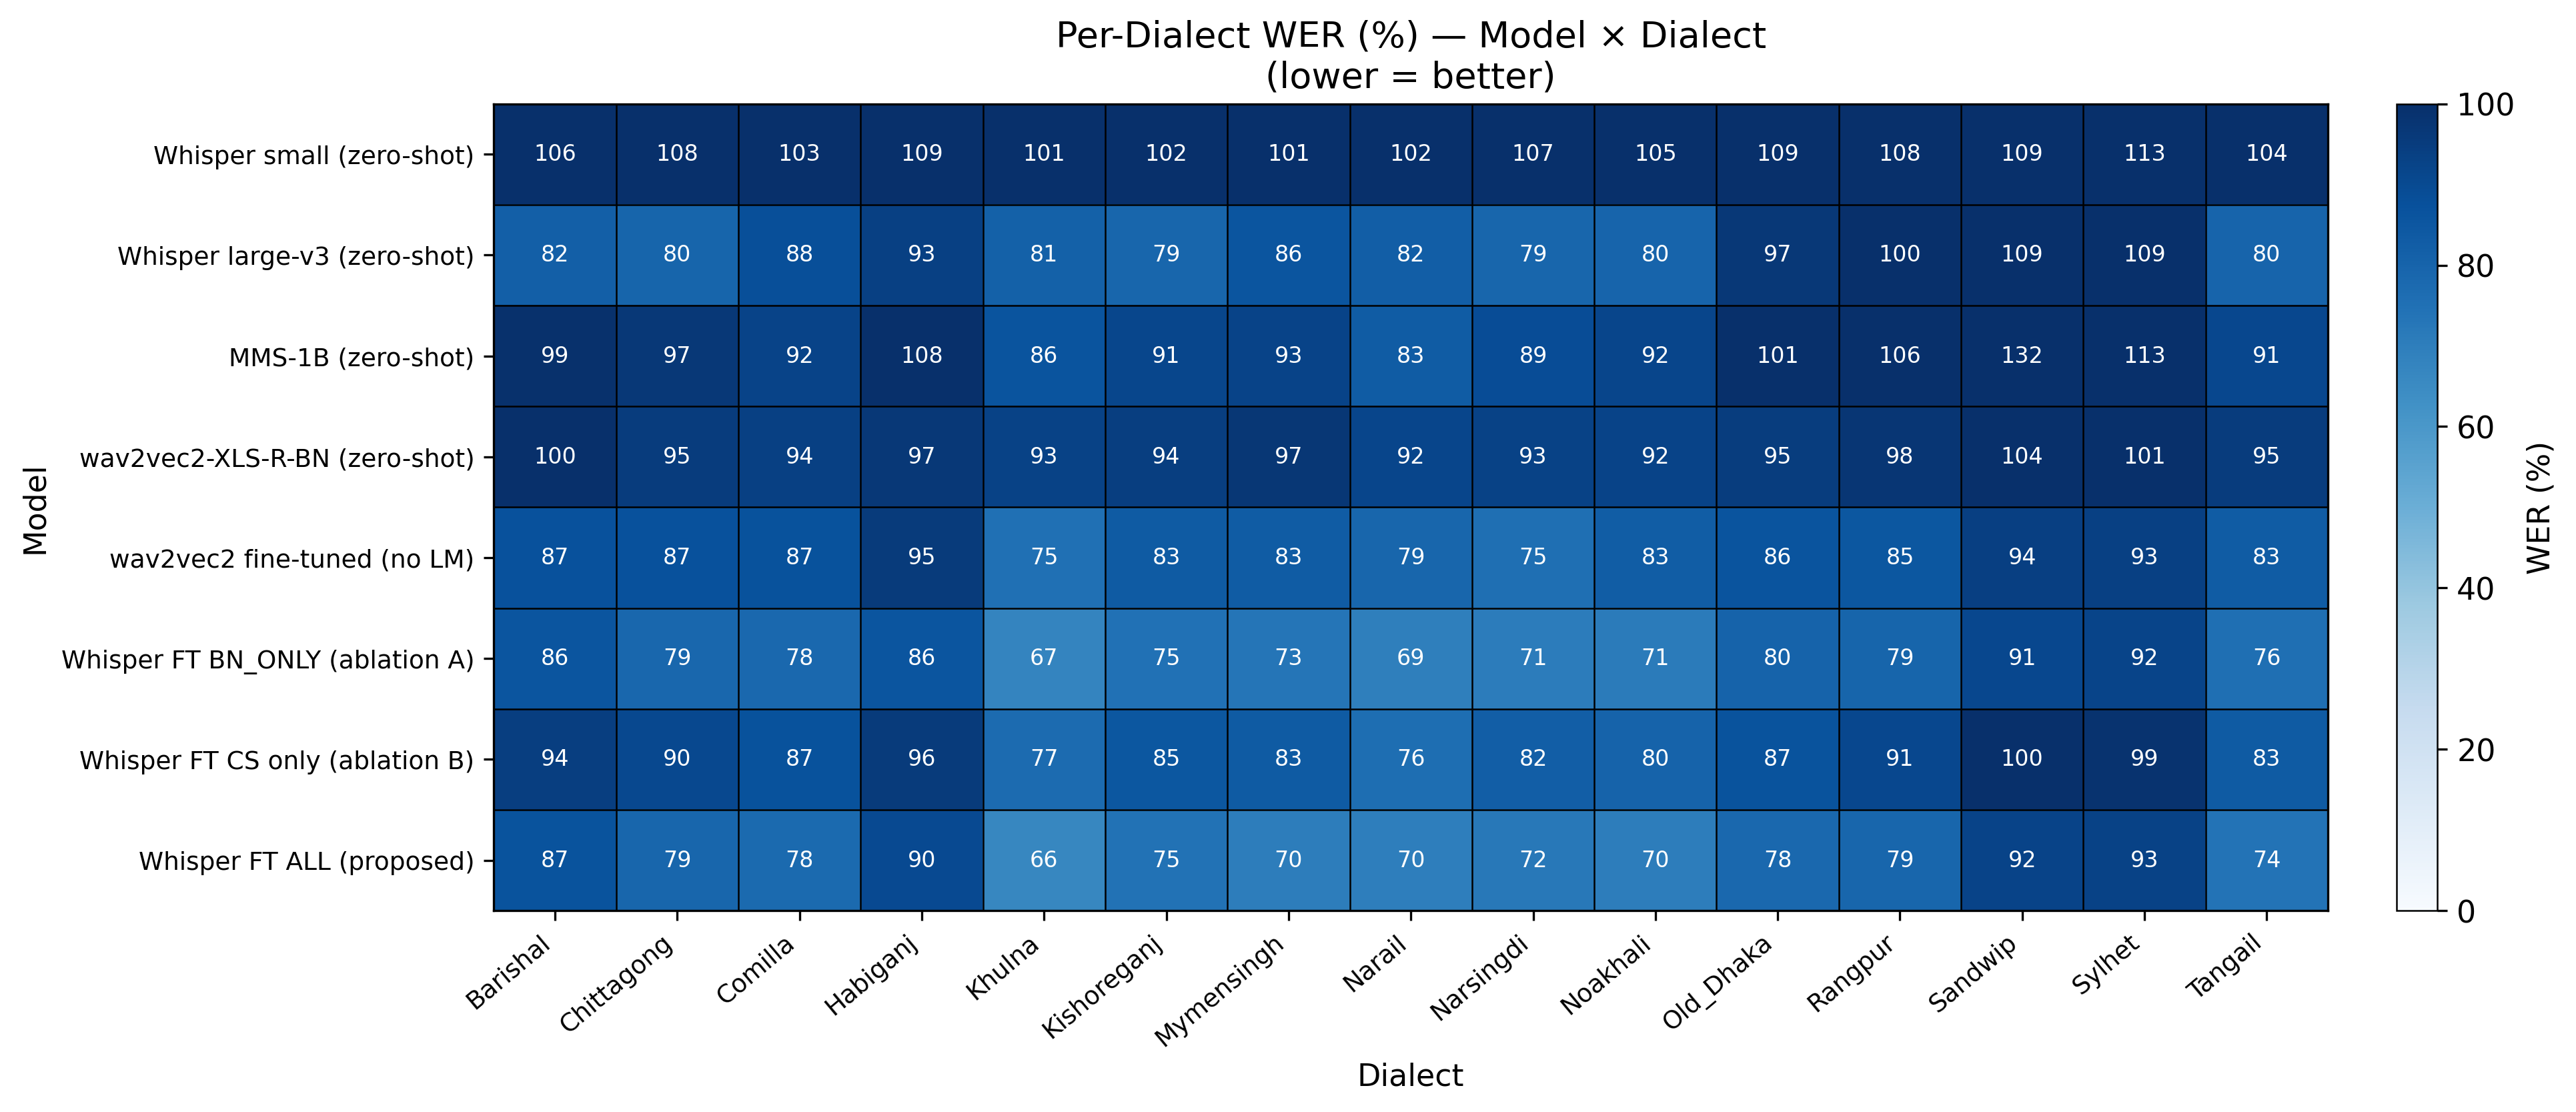
\includegraphics[width=\columnwidth]{figures/dialect_wer_heatmap.png}
\caption{Model $\times$ dialect WER heatmap.
Red = high WER, green = low WER.
Rows: models (baselines to proposed).
Columns: dialects.}
\label{fig:dialect_heatmap}
\end{figure}
